% This template has been tested with IEEEtran of 2015.
% Template from https://github.com/latextemplates/IEEE

% !TeX spellcheck = en-US
% !TeX encoding = utf8
% !TeX program = pdflatex
% !BIB program = bibtex
% -*- coding:utf-8 mod:LaTeX -*-

% To set up:
% aptitude install texlive-publishers texlive-lang-european texlive-latex-extra

% PBROWN: Use this to suppress the warning when including multiple matplotlib PDF plots on the same page
\pdfsuppresswarningpagegroup=1

%cmap has to be loaded before any font package (such as newtxmath)
\RequirePackage{cmap}

% DO NOT DOWNLOAD IEEEtran.cls - Use the one of your LaTeX distribution
% On Ubuntu, aptitude install texlive-publishers
\documentclass[conference,a4paper]{IEEEtran}[2015/08/26]

% use nicer font for code
\usepackage[zerostyle=b,scaled=.75]{newtxtt}

\usepackage[T1]{fontenc}
\usepackage[utf8]{inputenc} %support umlauts in the input
% I added the following to get Times Roman in math. Otherwise the g's looked really different.
% See https://tex.stackexchange.com/questions/9685/math-and-times-font#9686
\usepackage[italic]{mathastext}

\usepackage{graphicx}

\usepackage[inkscapelatex=false]{svg}

%Set English as language and allow to write hyphenated"=words
% For Turkish, on Ubuntu aptitude install texlive-lang-european
%\usepackage[english]{babel}
% If using Turkish, also set option shorthands=off
%Hint by http://tex.stackexchange.com/a/321066/9075 -> enable "= as dashes
%\addto\extrasenglish{\languageshorthands{ngerman}\useshorthands{"}}

% backticks (`) are rendered as such in verbatim environment. See https://tex.stackexchange.com/a/341057/9075 for details.
\usepackage{upquote}

%extended enumerate, such as \begin{compactenum}
\usepackage{paralist}

%for easy quotations: \enquote{text}
\usepackage{csquotes}

\usepackage{amsmath}

%enable margin kerning
\RequirePackage{iftex}
\ifPDFTeX
  \RequirePackage[%
    final,%
    expansion=alltext,%
    protrusion=alltext-nott]{microtype}%
\else
  \RequirePackage[%
    final,%
    protrusion=alltext-nott]{microtype}%
\fi%
% \texttt{test -- test} keeps the "--" as "--" (and does not convert it to an en dash)
\DisableLigatures{encoding = T1, family = tt* }

%tweak \url{...}
\usepackage{url}
%\urlstyle{same}
%improve wrapping of URLs - hint by http://tex.stackexchange.com/a/10419/9075
\makeatletter
\g@addto@macro{\UrlBreaks}{\UrlOrds}
\makeatother
%nicer // - solution by http://tex.stackexchange.com/a/98470/9075
%DO NOT ACTIVATE -> prevents line breaks
%\makeatletter
%\def\Url@twoslashes{\mathchar`\/\@ifnextchar/{\kern-.2em}{}}
%\g@addto@macro\UrlSpecials{\do\/{\Url@twoslashes}}
%\makeatother

% Diagonal lines in a table - http://tex.stackexchange.com/questions/17745/diagonal-lines-in-table-cell
% Slashbox is not available in texlive (due to licensing) and also gives bad results. This, we use diagbox
%\usepackage{diagbox}

\usepackage{booktabs}

% Required for package pdfcomment later
\usepackage{xcolor}

% For listings
\usepackage{listings}
\lstset{%
  basicstyle=\ttfamily,%
  columns=fixed,%
  basewidth=.5em,%
  xleftmargin=0.5cm,%
  captionpos=b}%

% Enable nice comments
\usepackage{pdfcomment}
%
\newcommand{\commentontext}[2]{\colorbox{yellow!60}{#1}\pdfcomment[color={0.234 0.867 0.211},hoffset=-6pt,voffset=10pt,opacity=0.5]{#2}}
\newcommand{\commentatside}[1]{\pdfcomment[color={0.045 0.278 0.643},icon=Note]{#1}}
%
% Compatibility with packages todo, easy-todo, todonotes
\newcommand{\todo}[1]{\commentatside{#1}}
% Compatiblity with package fixmetodonotes
\newcommand{\TODO}[1]{\commentatside{#1}}

% Bibliopgraphy enhancements
%  - enable \cite[prenote][]{ref}
%  - enable \cite{ref1,ref2}
% Alternative: \usepackage{cite}, which enables \cite{ref1, ref2} only (otherwise: Error message: "White space in argument")
%
% Doc: http://texdoc.net/natbib
\ifCLASSOPTIONcompsoc
  % IEEE Computer Society needs nocompress option at cite.sty
  % natbib includes the same functionality
  \usepackage[%
    square,        % for square brackets
    comma,         % use commas as separators
    numbers,       % for numerical citations;
    sort           % orders multiple citations into the sequence in which they appear in the list of references;
    %sort&compress % as sort but in addition multiple numerical citations
                   % are compressed if possible (as 3-6, 15);
  ]{natbib}
\else
  % normal IEEE
  \usepackage[%
    square,        % for square brackets
    comma,         % use commas as separators
    numbers,       % for numerical citations;
    %sort           % orders multiple citations into the sequence in which they appear in the list of references;
    sort&compress % as sort but in addition multiple numerical citations
                   % are compressed if possible (as 3-6, 15);
  ]{natbib}
\fi
% Same fontsize as without natbib
\renewcommand{\bibfont}{\normalfont\footnotesize}

% Enable hyperlinked author names in the case of \citet
% Source: https://tex.stackexchange.com/a/76075/9075
\usepackage{etoolbox}
\makeatletter
\patchcmd{\NAT@test}{\else \NAT@nm}{\else \NAT@hyper@{\NAT@nm}}{}{}
\makeatother

% Enable that parameters of \cref{}, \ref{}, \cite{}, ... are linked so that a reader can click on the number an jump to the target in the document
\usepackage{hyperref}
% Enable hyperref without colors and without bookmarks
\hypersetup{hidelinks,
  colorlinks=true,
  allcolors=black,
  pdfstartview=Fit,
  breaklinks=true}
%
% Enable correct jumping to figures when referencing
\usepackage[all]{hypcap}

%\renewcommand{\figurename}{Fig.}

%enable \cref{...} and \Cref{...} instead of \ref: Type of reference included in the link
\usepackage[capitalise,nameinlink]{cleveref}
%\crefname{lstlisting}{\lstlistingname}{\lstlistingname}
%\Crefname{lstlisting}{Listing}{Listings}
% The following are to comply with the IEEE style guide.
\crefformat{equation}{#2(#1)#3}
\Crefformat{equation}{#2Equation #1#3}
\crefname{figure}{Fig.}{Figs.}
%\Crefname{figure}{Fig.}{Figs.}

%Following definitions are outside of IfPackageLoaded; inside, they are not visible
%
%Intermediate solution for hyperlinked refs. See https://tex.stackexchange.com/q/132420/9075 for more information.
\newcommand{\Vlabel}[1]{\label[line]{#1}\hypertarget{#1}{}}
\newcommand{\lref}[1]{\hyperlink{#1}{\FancyVerbLineautorefname~\ref*{#1}}}

\newenvironment{listing}[1][htbp!]{\begin{figure}[#1]}{\end{figure}}
\newcounter{listing}

\usepackage{xspace}
%\newcommand{\eg}{e.\,g.\xspace}
%\newcommand{\ie}{i.\,e.\xspace}
\newcommand{\eg}{e.\,g.,\ }
\newcommand{\ie}{i.\,e.,\ }

%introduce \powerset - hint by http://matheplanet.com/matheplanet/nuke/html/viewtopic.php?topic=136492&post_id=997377
\DeclareFontFamily{U}{MnSymbolC}{}
\DeclareSymbolFont{MnSyC}{U}{MnSymbolC}{m}{n}
\DeclareFontShape{U}{MnSymbolC}{m}{n}{
  <-6>    MnSymbolC5
  <6-7>   MnSymbolC6
  <7-8>   MnSymbolC7
  <8-9>   MnSymbolC8
  <9-10>  MnSymbolC9
  <10-12> MnSymbolC10
  <12->   MnSymbolC12%
}{}
\DeclareMathSymbol{\powerset}{\mathord}{MnSyC}{180}

% *** SUBFIGURE PACKAGES ***
\ifCLASSOPTIONcompsoc
  \usepackage[caption=false,font=footnotesize,labelfont=sf,textfont=sf]{subfig}
\else
  \usepackage[caption=false,font=footnotesize]{subfig}
\fi

\usepackage{stfloats}



% correct bad hyphenation here
\hyphenation{op-tical net-works semi-conduc-tor}

\graphicspath{{./figs/}}

% Paper-specific packages that I have added:
\usepackage{siunitx}  % For units with \SI
\usepackage{threeparttable}  % For tablenotes
\usepackage{placeins}  % For \FloatBarrier
\usepackage{xfrac}  % For \sfrac
%\usepackage{orcidlink}  % For orcid link
\DeclareMathOperator{\logicand}{and}
\DeclareMathOperator{\logicor}{or}


%\bibliographystyle{chicago}   % For drafts only, to make it easier to see which references have been used.
\bibliographystyle{IEEEtranN} % IEEEtranN is the natbib compatible bst file
%\usepackage{showkeys}          % For drafts only


\begin{document}
%\IEEEoverridecommandlockouts

\title{Operational Optimization of an Agricultural Microgrid}

\author{%
  \IEEEauthorblockN{Paul Brown}
  
  \IEEEauthorblockA{2463461\\
   ***REMOVED***}
}

% use for special paper notices
%\IEEEspecialpapernotice{(Invited Paper)}

% make the title area
\maketitle

% In case you want to add a copyright statement.
%
% Source: https://tex.stackexchange.com/a/200330/9075
%
% All possible solutions:
%  - https://tex.stackexchange.com/a/325013/9075
%  - https://tex.stackexchange.com/a/279134/9075
%  - https://tex.stackexchange.com/q/279789/9075 (TikZ)
%  - https://tex.stackexchange.com/a/200330/9075 - for non-compsocc papers
\iffalse
    \makeatletter
    \def\ps@IEEEtitlepagestyle{%
      \def\@oddfoot{\mycopyrightnotice}%
      \def\@evenfoot{}%
    }
    \makeatother
    \def\mycopyrightnotice{%
      \begin{minipage}{\textwidth}
        \footnotesize
        1551-3203 \copyright 2015 IEEE.
        Personal use is permitted, but republication/redistribution requires IEEE permission.
        \\
        See \url{https://www.ieee.org/publications_standards/publications/rights/index.html} for more information.
      \end{minipage}
      \gdef\mycopyrightnotice{}% just in case
    }
\fi

\begin{abstract}
  A demonstration agricultural microgrid containing PV, battery energy storage (BSS) and multiple water pumps is presented.
A mathematical model of the cost of operating the microgrid is developed, including modeling of battery charging modes and hybrid inverter source selection.
The mathematical model is implemented in Python using Pyomo and optimized to plan pumping and water usage.
The model may serve as the basis for model predictive control (MPC) or stochastic model predictive control (SMPC).
\end{abstract}

\begin{IEEEkeywords}
	Microgrid, optimization, photovoltaic systems, energy storage, irrigation
\end{IEEEkeywords}

% For peer review papers, you can put extra information on the cover
% page as needed:
% \ifCLASSOPTIONpeerreview
% \begin{center} \bfseries EDICS Category: 3-BBND \end{center}
% \fi
%
% For peerreview papers, this IEEEtran command inserts a page break and
% creates the second title. It will be ignored for other modes.
\IEEEpeerreviewmaketitle

\section{Introduction}
\label{sec:intro}

\IEEEPARstart{T}{his} is the introduction. This topic is about something really important. I should probably include a lot of references here. This is the place to show some literature review.



% Make sure any figures start AFTER the introduction and don't float above it.
\FloatBarrier

\section{Demonstration System}
\label{sec:demo-system}

The optimization problem is specifically formulated for a demonstration system to be installed at the Güneşköy farm\cite{Guneskoy}. A block diagram of the demonstration system is shown in \cref{fig:demo-system}.

The existing pump will continue to be fed from the grid. The site electrical load will be fed from a hybrid inverter\cite{INVT_manual} that will have battery, PV, and grid connections available. A new pump load will be fed from an inverter drive\cite{Growatt_manual} connected to the PV DC bus.

\begin{figure}[t]
	\centering
	\fontsize{6.7pt}{9pt}\selectfont
	\def\svgwidth{0.8\columnwidth}
	\input{figs/demo_system.pdf_tex}
	\caption{Güneşköy Demonstration System}
	\label{fig:demo-system}
\end{figure}

The power flows within the demonstration system are shown in \cref{fig:power-flows}.

\begin{figure}[t]
	\centering
	\input{figs/power_flows.pdf_tex}
	\caption{Microgrid power flows}
	\label{fig:power-flows}
\end{figure}







\section{Problem formulation}
\label{sec:problem-formulation}

\autoref{table:variables} shows problem variables that are to be determined by the optimization process.
\autoref{table:calculated} shows quantities that are calculated based on the problem equations.

\subsection{Problem variables}



\begin{table}[htb]
	\begin{threeparttable}[b]
		\caption{Problem variables}
		\label{table:variables}
		\begin{tabular}{cp{0.7\columnwidth}c}
			\toprule 
			Symbol & Description & Units \\
			\midrule
			$s_{pump1,t}$ & Pump 1 on-off selection variable\tnote{2} & - \\
			$P_{pump2,t}$ & Power used for pumping water to Reservoir 2 & \si{W} \\
			$Q_{use1,t}$ & Flow of water used (irrigation or other use) from Reservoir 1 & \si{m^3/h} \\
			$Q_{use2,t}$ & Flow of water used (irrigation or other use) from Reservoir 2 & \si{m^3/h} \\
			\bottomrule
		\end{tabular}
		\begin{tablenotes}
			\footnotesize
			\item [1] Variables subscripted with $t$ have a value for each time period
			\item [2] Binary variable. 1: Running. 0: Off.
		\end{tablenotes}
	\end{threeparttable}
\end{table}

\begin{table}[htb]
	\begin{threeparttable}[b]
		\caption{Calculated quantities}
		\label{table:calculated}
		\begin{tabular}{cp{0.6\columnwidth}c}
			\toprule 
			Symbol & Description & Units \\
			\midrule
			$P_{pump1,t}$ & Power used by Pump 1 for pumping water to Reservoir 1 & \si{W} \\
			$Q_{pump1,t}$ & Volume of water pumped by Pump 1 & \si{m^3} \\
			%$s_{pump2,on,t}$ & Pump on-off selection variable\tnote{2} & - \\
			%$P_{pump2,t}$ & Power used by Pump 2 for pumping water to Reservoir 2 & \si{W} \\
			$Q_{pump2,t}$ & Volume of water pumped by Pump 2 & \si{m^3} \\
			$s_{BSS,t}$ & Operating mode of BSS\tnote{3} & - \\
			$P_{BSS,ch,t}$ & Power used to charge the BSS & \si{W} \\
			$P_{BSS,disch,t}$ & Power drawn from discharging the BSS & \si{W} \\
			$s_{inv,t}$ & Inverter mode\tnote{4} & - \\
			$P_{PV,t}$ & Power drawn from the PV array & \si{W} \\
			%$P_{avail,t}$ & Available PV power minus load on microgrid & \si{W} \\
			$P_{PV-inverter,t}$ & Power flow from the PV bus to the inverter & \si{W} \\
			$P_{grid,t}$ & Power drawn from the electrical grid or load not served & \si{W} \\
			$P_{grid-inverter,t}$ & Power drawn from the grid to feed the hybrid inverter & \si{W} \\
			$E_{BSS,t}$ & Energy stored in the BSS at the end of the period & \si{W h} \\
			$V_{w1,t}$ & Volume of water stored in the Reservoir 1 at the end of the period & \si{m^3} \\
			$V_{w2,t}$ & Volume of water stored in the Reservoir 2 at the end of the period & \si{m^3} \\
			$V_{use,d}$ & Effectively used volume of water (irrigation or other use) on day $d$ & \si{m^3} \\
			\bottomrule
		\end{tabular}
		\begin{tablenotes}
			\footnotesize
			\item [1] Variables subscripted with $t$ have a value for each time period
			\item [2] Binary variable. 1: Running. 0: Off.
			\item [3] Binary variable. 1: Charging. 0: Discharging.
			\item [4] Binary variable. 1: Inverter fed from utility source. 0: Inverter fed from BSS/PV source.
		\end{tablenotes}
	\end{threeparttable}
\end{table}


\begin{table}[htb]
	\begin{threeparttable}[b]
		\caption{Problem parameters / data}
		\label{table:parameters}
		\begin{tabular}{cp{0.6\columnwidth}c}
			\toprule 
			Symbol & Description & Units \\
			\midrule
			$P_{load,t}$ & Power drawn by electrical loads & \si{W} \\
			$P_{PV,avail,t}$ & Power available from PV array (MPP) & \si{W} \\
			$P_{pump1,max}$ & Operating power of Pump 1 & \si{W} \\
			$s_{pump1,0}$ & Initial state of Pump 1 & - \\
			$Q_{w1}$ & Fixed water flow for Pump 1 & \si{m^3 / h} \\
			$P_{pump2,min}$ & Minimum operating power of Pump 2 & \si{W} \\
			$P_{pump2,max}$ & Maximum operating power of Pump 2 & \si{W} \\
			$Q_{w2}\left(P_{pump2}\right)$ & Function relating pumped water quantity to electrical power for Pump 2 & \si{m^3 / h} \\
			$P_{BSS,ch,max}$ & Bulk charging power for the BSS & \si{W} \\
			$P_{BSS,disch,max}$ & Maximum power for discharging the BSS & \si{W} \\
			$K_{BSS}$ & BSS absorption mode charge rate constant (0 - 1) & - \\
			$E_{BSS,0}$ & Initial value of energy stored in the BSS & \si{W h} \\
			$s_{inv,0}$ & Initial state of inverter & - \\
			$E_{BSS,max}$ & Maximum energy that can be stored in the BSS & \si{W h} \\
			$E_{BSS,lower}$ & Inverter threshold to switch from BSS/PV source to utility source & \si{W} \\
			$E_{BSS,upper}$ & Inverter threshold to switch from utility source to BSS/PV source & \si{W} \\
			$V_{w1,0}$ & Initial value of water stored in Reservoir 1 & \si{m^3} \\
			$V_{w1,min}$ & Minimum volume of water that can be stored in Reservoir 1 & \si{m^3} \\
			$V_{w1,max}$ & Maximum volume of water that can be stored in Reservoir 1 & \si{m^3} \\
			$V_{w2,0}$ & Initial value of water stored in Reservoir 2 & \si{m^3} \\
			$V_{w2,min}$ & Minimum volume of water that can be stored in Reservoir 2 & \si{m^3} \\
			$V_{w2,max}$ & Maximum volume of water that can be stored in Reservoir 2 & \si{m^3} \\
			$V_{use,desired,d}$ & Desired volume of effectively used water on day $d$& \si{m^3} \\
			$D_d$ & Set of time periods $t$ belonging to day $d$. & - \\
			$Q_{use1,max}$ & Maximum rate of water use from Reservoir 1 & \si{m^3 / h} \\
			$Q_{use2,max}$ & Maximum rate of water use from Reservoir 2 & \si{m^3 / h} \\
			$C_{grid,t}$ & Cost of power from the grid & \si{\$ / W h} \\
			$C_{BSS}$ & Cost of storing power in the BSS & \si{\$ / W h} \\
			$C_{BSS,switching}$ & Penalty for changing BSS charging/discharging mode & \si{\$/ea} \\
			$C_{w,short}$ & Cost or penalty factor for water that is desired but not used & \si{\$ / m^3} \\
			$\eta_{BSS}$ & Efficiency of BSS in charging or discharging & - \\
			$\eta_{w,t}$ & Efficiency of water use & - \\
			$\Delta t$ & Time interval for discretized planning horizon & \si{h} \\
			\bottomrule
		\end{tabular}
		\begin{tablenotes}
			\footnotesize
			\item [1] Variables subscripted with $t$ have a value for each time period
		\end{tablenotes}
	\end{threeparttable}
\end{table}

\subsection{Objective function}

The objective function includes several components and is shown in \autoref{eqn:objective-function}. The actual cost component is cost of grid power. The cost of battery usage component represents the portion of the replacement cost of the battery system incurred due to the loss of life caused by battery cycling. The other penalty factors encourage the full supply of desired water on each day and discourage unnecessary switching of the BSS mode and Pump 1 respectively.
%
\begin{equation}
\label{eqn:objective-function}
\begin{split}
\min &\underbrace{\sum_t C_{grid,t} \ P_{grid,t} \ \Delta t}_{\textrm{Cost of grid power}}
+ \underbrace{\sum_t C_{BSS} \left( P_{BSS,ch,t} + P_{BSS,disch,t} \right) \Delta t}_{\textrm{Cost of battery usage}}
\\
+ &\underbrace{C_{w,short} \sum_d \max\left(\left(V_{use,desired,d} - V_{use,d}\right), 0\right)}_{\textrm{Penalty for inadequate water}}
\\
+ &\underbrace{C_{BSS,switching} \sum_t \left| s_{BSS,t} - s_{BSS,t-1} \right|}_{\textrm{BSS mode-switching penalty}}
\\
+ &\underbrace{C_{Pump1,switching} \sum_t \left| s_{pump1,t} - s_{pump1,t-1} \right|}_{\textrm{Pump 1 switching penalty}}
\end{split}
\end{equation}


\subsection{Constraints}

\subsubsection{Power Balance}

There is a power balance constraint equation for each of the four buses shown in \autoref{fig:power-flows}. \autoref{eqn:power-balance-PV} enforces balance on the PV bus, \autoref{eqn:power-balance-inverter} enforces balance in the hybrid inverter PV/BSS side, \autoref{eqn:power-balance-inverter-grid} enforces balance in the hybrid inverter grid side, and \autoref{eqn:power-balance-grid} enforces balance on the grid-side bus.
%
\begin{gather}
\label{eqn:power-balance-PV}
P_{PV,t} - P_{pump2,t} - P_{PV-inverter,t} = 0 \\
\label{eqn:power-balance-inverter}
\begin{split}
P_{PV-inverter,t} + P_{BSS,disch,t}& - P_{BSS,ch,t} \\
 &- \left( 1 - s_{inv,t}\right) \ P_{load,t} = 0 
\end{split}
\\
\label{eqn:power-balance-inverter-grid}
P_{grid-inverter,t} = s_{inv,t} \ P_{load,t} \\
\label{eqn:power-balance-grid}
P_{grid,t} - P_{grid-inverter,t} - P_{pump1,t} = 0
\end{gather}

The direction of power flow from the PV bus to the inverter and from the grid to the inverter must be constrained to be positive.
%
\begin{gather}
\label{eqn:pv-inverter-positive}
0 \le P_{PV-inverter,t} \\
\label{eqn:grid-inverter-positive}
0 \le P_{grid-inverter,t}
\end{gather}

\subsubsection{Photovoltaic}

It is assumed that the microgrid has the ability to track the photovoltaic array maximum power point (MPP) regardless of the operation of either or both of the hybrid inverter and the drive for Pump 2. It is also assumed that the control system has the ability to know what the maximum available PV power is, even if the system is not operating at the MPP. The full available output of the PV system may not be used if the load is less than the available PV power.
%
\begin{equation}
\label{eqn:pv-limit}
0 \le P_{PV,t} \le P_{PV,avail,t}
\end{equation}

\subsubsection{Pumps}

Pump 1 is operated in a simple on-off fashion at a fixed power level.
%
\begin{gather}
\label{eqn:pump1-power}
P_{pump1,t} = s_{pump1,t} \ P_{pump1,max} \\
\label{eqn:pump1-flow}
Q_{pump1,t} = s_{pump1,t} \ Q_{w1}
\end{gather}

It is assumed that Pump 2 may be operated at a specified range-limited setpoint chosen by the controller. The pumping power $P_{pump2,t}$ is a semi-continuous variable, being continuous between a minimum and a maximum or else 0.
%
\begin{gather}
\label{eqn:pump2-power}
P_{pump2,t} = 0 \ \lor \ P_{pump2,min} \le P_{pump2,t} \le P_{pump2,max} \\
\label{eqn:pump2-flow}
Q_{pump2,t} = Q_{w2}\left( P_{pump2,t} \right)
\end{gather}

\autoref{eqn:pump-flow-relation} is a placeholder for the currently unknown relationship between pump flow and power. For real-time control, the EMS controller could infer this relationship by observing the operation of the pump. Until then, a simple linear efficiency coefficient $\eta_{pump2}$ is used to characterize the power-flow relationship of Pump 2.
%
\begin{equation}
\label{eqn:pump-flow-relation}
 Q_{w2}\left( P_{pump2,t} \right) = \frac{P_{pump2,t} \ \eta_{pump2}}{h \rho g}
\end{equation}

\subsubsection{Hybrid Inverter and BSS}

The hybrid inverter selected for the demonstration system at Güneşköy has limited capability to receive external control. It is assumed that the hybrid inverter will be configured with a priority order for supplying load such that the load will be supplied from PV if available, supplemented by power from the BSS. If PV is not sufficient and the BSS charge level is too low, then the utility grid source will be used. It is assumed that the hybrid inverter will charge the BSS only from PV and not from the utility grid source.

It is planned for the BSS to consist of lead-acid batteries. The hybrid inverter is responsible for charging the lead-acid battery bank. The inverter uses a four-stage charging cycle:

\begin{enumerate}
	\item \textbf{Bulk charging.} Charges at a settable maximum charging current. The power to the battery is nearly constant and is approximated in this formulation as a constant power $P_{BSS,ch,max}$.
	\item \textbf{Absorption charging.} Once the voltage reaches set maximum charging voltage, the voltage is held for a duration of 10 times the time spent in bulk charging mode. The power to the battery declines exponentially with time as the BSS voltage approaches the charging voltage and the SOC approaches 100\%.
	\item \textbf{Float charging.} Once the absorption charge timer completes, the charger switches to float charging mode in which a fixed voltage is held and minimal charging current is output except to compensate the small battery internal discharge or small load discharging of the battery.
	\item \textbf{Equalization charging.} Equalization charging is only applicable to flooded lead acid batteries and not to sealed lead acid batteries. In this mode, the battery is temporarily overcharged in order to reduce sulfation on the battery plates.
\end{enumerate}

For the purposes of a mathematical model of the hybrid inverter's battery charging system for this optimization problem, only the bulk charging and absorption charging modes are represented. The other charging modes are neglected since most of the energy transfer to the BSS is completed these modes.

\autoref{eqn:sBSS} forces the charger state to charge if power is available.
\autoref{eqn:BSS-mode-charging} enforces the limit for absorption charging mode of the hybrid inverter,
limits charging power to available power from the PV after meeting pumping and load power,
and only allows charging when $s_{BSS,t}$ is in charging mode.
\autoref{eqn:BSS-mode-discharging} only allows discharging when $s_{BSS,t}$ is in discharging mode.
%
\begin{gather}
\label{eqn:sBSS}
s_{BSS,t} = \left( P_{PV,avail,t} - P_{pump2,t} - (1 - s_{inv,t}) P_{load,t} \ge 0 \right)
\\
\label{eqn:BSS-mode-charging}
\begin{aligned}
P_{BSS,ch,t} = \min\Big(
& \underbrace{K_{BSS} \ \frac{E_{BSS,max} - E_{BSS,t-1}}{\eta_{BSS} \ \Delta t}}_
{\textrm{Absorption mode charging limit}},
\\
& \underbrace{P_{PV,avail,t} - P_{pump2,t} - (1 - s_{inv,t}) P_{load,t}}_
{\textrm{Unused available PV power}},
\\
& \underbrace{s_{BSS,t} \ P_{BSS,ch,max}}_  
{\textrm{Enforce charger mode}} \Big)
\end{aligned}
\\
\label{eqn:BSS-mode-discharging}
0 \le P_{BSS,disch,t} \le \left(1 - s_{BSS,t}\right) P_{BSS,disch,max}
\end{gather}

The constant $K_{BSS}$ takes a value between 0 and 1 and determines this switchover point from bulk charging mode to absorption charging and the rate of decrease in the charging power in absorption charging mode. A $K_{BSS}$ value of 1 indicates that the charger remains in bulk charging mode until the BSS is fully charged. The value of $K_{BSS}$ can be related to the time constant of the exponential decay of charging power in absorption mode, $\tau_{BSS}$ as shown in \autoref{eqn:calculate-K-BSS}. This relationship can be used to calculate $K_{BSS}$ or to convert a known $K_{BSS}$ from one modeling time interval $\Delta t$ to another.
%
\begin{equation}
\label{eqn:calculate-K-BSS}
K_{BSS} = 1 - e^{\sfrac{-\Delta t}{\tau_{BSS}}}
\end{equation}

According to the the hybrid inverter user manual, when in ``SBU priority'' mode, the hybrid inverter switches from PV/battery source to utility source when the battery goes below a minimum voltage level and switches back to the battery when the battery rises above a minimum voltage level. \autoref{eqn:inverter-mode} represents this logic to determine the connection of the inverter in time period $t$ based on the connection during the previous period and the BSS energy level at the end of the previous period. In this way of modeling, the mode is switched only at discrete time intervals, so the model will show the battery BSS charge level will going a little above and below the set thresholds rather than switching mid-period as the actual hybrid inverter will do.
%
\begin{equation}
\label{eqn:inverter-mode}
\begin{split}
s_{inv,t} = \left(s_{inv,t-1} \logicand \left(E_{BSS,t-1} \le E_{BSS,upper} \right) \right)
\logicor
\\
\left( E_{BSS,t-1} \le E_{BSS,lower} \right)
\end{split}
\end{equation}

\autoref{eqn:BSS-balance} couples the battery system energy balance from one period to the next. It includes a factor for conversion losses on energy input and energy output. An alternative formulation would be to make the efficiency factor be ``round trip'' and only include it on one of charging or discharging power rather than both.
%
\begin{equation}
\label{eqn:BSS-balance}
E_{BSS,t} = E_{BSS,t-1} + P_{BSS,ch,t} \ \eta_{BSS} \ \Delta t - \frac{P_{BSS,disch,t} \ \Delta t}{\eta_{BSS}}
\end{equation}

\subsubsection{Water Flow}

\autoref{eqn:water-balance-1} and \autoref{eqn:water-balance-2} couple the water level in Reservoir 1 and Reservoir 2 from one period to the next. It does not include water losses at this time, but water losses could be incorporated into this equation in the future.
%
\begin{gather}
\label{eqn:water-balance-1}
V_{w1,t} = V_{w1,t-1} + Q_{pump1,t} \ \Delta t - Q_{use1,t} \Delta t \\
\label{eqn:water-balance-2}
V_{w2,t} = V_{w2,t-1} + Q_{pump2,t} \ \Delta t - Q_{use2,t} \Delta t
\end{gather}

\autoref{eqn:total-water} sums the effective irrigation water across periods in each day, taking into consideration the varying efficiency of irrigation in different periods.
It is assumed that water use between the two reservoirs is interchangeable.
%
\begin{equation}
\label{eqn:total-water}
V_{use,d} = \sum_{t \in D_d}  \eta_{w,t} \left( Q_{use1,t} +  Q_{use2,t} \right) \Delta t
\end{equation}

Equations \ref{eqn:var-limit-1st} through \ref{eqn:var-limit-last} are the limits on feasible values of the water flow and reservoir level values.
%
\begin{gather}
\label{eqn:var-limit-1st}
0 \le Q_{use1,t} \le Q_{use1,max} \\
0 \le Q_{use2,t} \le Q_{use2,max} \\
V_{w1,min} \le V_{w1,t} \le V_{w1,max} \\
\label{eqn:var-limit-last}
V_{w2,min} \le V_{w2,t} \le V_{w2,max}
\end{gather}




\section{Data Values}

Data for the problem parameters was estimated based on the planned demonstration system shown in \cref{fig:demo-system}.
While the parameters used are intended to represent a realistic system, they have not been validated operationally.
%Nonetheless, they should suffice to illustrate the proposed mathematical model.
Rather than providing data values for all the problem parameters shown in \cref{table:parameters}, due to space limitations, a more general description of the parameters selection is given.

Grid energy costs $C_{grid,t}$ were set for the daytime, peak, and nighttime rates and daily periods that Güneşköy was billed at in 2020, not including fees for power factor, etc.

Water usage efficiency $\eta_{w,t}$ was set using different values for each hour of the day, with the highest efficiency (\num{1.0}) during nighttime hours and the lowest efficiency (\num{0.5}) during early afternoon.

Random values were generated for the load and the desired water use. Load was drawn from a uniform distribution ranging from 0 to \SI{1}{kW}.
Daily desired water use was drawn from a normal distribution with a mean of \SI{70}{m^3} and a standard deviation of \SI{30}{m^3}.

Pump, battery, and PV parameters were selected to represent the demonstration system shown in \cref{fig:demo-system}.
The hybrid inverter source selection was configured to stay on the PV/BSS source until the BSS charge dropped below 30\% and then switch to the grid to charge until it reached a charge level of 95\%.
The BSS charging and discharging efficiency was set to 95\%.
Hourly averages of the recorded output power of the rooftop PV array on the METU EEE Department machinery building were scaled to the rating of the demonstration system and used for the available PV power.

The optimization period was set for a length of \SI{72}{h} with a time step $\Delta t$ of \SI{1}{h} used. The time period of \SI{72}{h} (3 days) was used so that the optimizer wouldn't use up all the stored water and energy to meet the needs of the first day, neglecting its benefit for future days.
Initial values for $E_{BSS}$, $V_{w1}$, $V_{w2}$, and $s_{inv}$ were set arbitrarily for the first period optimized.
For subsequent periods, the time period being optimized was slid forward by \SI{24}{h}, and the value for the 24th hour of the previous period was used as the initial value for the current period.
The results shown in \cref{sec:results} are from the fourth in this series of sliding optimization runs.

\section{Implementation}

The problem was modeled in the Python programming language using the Pyomo library\cite{hart2011pyomo,bynum2021pyomo} and solved using the COIN-OR CBC\cite{CBC} open-source mixed-integer linear program (MILP) solver. In order to use a MILP solver, auxiliary binary variables were introduced to linearize non-linear functions such as $\max$, $\min$, absolute value, $\ge$, $\le$, and logic functions $\logicand$ and $\logicor$. The formulation of the non-linear functions was based on \cite{YALPMIP_logic} and original work by the author. Semi-continuous variables were modeled using the approach described in \cite{MILP_handout}.

% Problem size from logs saved with run 20220317_1333.
The problem, solved for a time period of \SI{72}{h} with an interval $\Delta t$ of \SI{1}{h}, contained a total of 566 continuous and 1008 binary variables. CBC converges to a solution in less than 30 seconds.

Initialization to a feasible point was performed using a single forward-pass heuristic of greedy pumping with Pump 2 if PV was available, then meeting loads with PV and BSS energy, discharging BSS to meet loads if necessarily and energy was available. Initial Pump 1 pumping and water use was set by iteratively solving a linear problem to try to add pumping one hour at a time until the desired water usage was met. The linear problem was implemented in Pyomo and solved using GLPK\cite{GLPK}.

\section{Results}
\label{sec:results}

The optimization run reduced the cost of the objective function from the initialized value of of \$\num{2655.7} to an optimized value of \$\num{1526.5}. The components of the initialized and optimized objective function costs are shown in \cref{table:optimal-costs}.
The proposed model improves upon a simple priority-based heuristic by allowing the optimizer to minimize the operating cost by pumping water or BSS charging or some of both.


\begin{table}[t]
	\caption{Objective Function Components}
	\label{table:optimal-costs}
	\centering
	\begin{tabular}{lS[table-format=5.1]S[table-format=5.1]}
		\toprule
		   & {Initialized}  & {Optimized} \\
		   &  {(\$, 2020)}     & {(\$, 2020)} \\
		\midrule
		Grid energy cost  &  2448.1  &  1192.4 \\
		Battery use cost  &  198.6  &  326.1 \\
		Inadequate water cost  & 0.0  &  0.0 \\
		Battery mode switching cost  &  8.0  &  7.0 \\
		Pump switching cost  &  1.0  &  2.0 \\
		\midrule
		TOTAL  &  2655.7  &  1526.5 \\
		\bottomrule		
	\end{tabular}
\end{table}

%Figures \ref{fig:pv-side-power} - \ref{fig:water-used} show the results of the optimization run.


\begin{figure}[t]
	\centering
	\includegraphics[page=2, clip, trim=0.05in 2.2in 7.2in 0.15in, width=1.0\columnwidth]{optimization_plots}
	\caption{PV-Side Power}
	\label{fig:pv-side-power}
\end{figure}

\Cref{fig:pv-side-power} shows the power on the PV and BSS side of the microgrid.
Due to the relative ratings of the PV array, Pump 2, and the BSS, on the sunny days (24 and 26 February), the full available PV power is not able to be used.
The optimal operation does not strictly prefer pumping water or charging the BSS.
Instead, the BSS is charged enough to prevent the hybrid inverter from switching back to the grid.


\begin{figure}[t]
	\centering
	\includegraphics[page=2, clip, trim=0.03in 0.55in 7.2in 2.3in, width=1.0\columnwidth]{optimization_plots}
	\caption{Grid-Side Power}
	\label{fig:grid-side-power}
\end{figure}

\begin{figure}[t]
	\centering
	% trim=left botm right top
	\includegraphics[page=2, clip, trim=3.7in 2.7in 3.55in 0.15in, width=1.0\columnwidth]{optimization_plots}
	\caption{BSS Energy Stored}
	\label{fig:bss-energy}
\end{figure}

\Cref{fig:grid-side-power} shows the power on the grid side of the microgrid.
On the first day (24 February), the hybrid inverter starts initially connected to the grid.
As shown in \cref{fig:bss-energy}, once the BSS is recharged by PV during the day, the hybrid inverter switches to the PV/BSS source and is able to supply the load for the rest of the modeled period.
The largest load on the grid is Pump 1, which optimally runs during the nighttime hours where time-of-day electrical rates are cheapest.


%\begin{figure}[t]
%	\centering
%	% trim=left botm right top
%	\includegraphics[page=4, clip, trim=3.3in 0.15in 3.9in 2.35in, width=1.0\columnwidth]{optimization_demo}
%	\caption{BSS Power (Charging \& Discharging)}
%	\label{fig:bss-power}
%\end{figure}
%
%\Cref{fig:bss-power} shows the charging and discharging power to the BSS.
%As one would expect, it follows a pattern of charging during the part of the day in which PV energy is available and discharging to meet load during the dark period.


\begin{figure}[t]
	\centering
	% trim=left botm right top
	\includegraphics[page=2, clip, trim=7.2in 2.9in 0.05in 0.15in, width=1.0\columnwidth]{optimization_plots}
	\caption{Water Stored}
	\label{fig:water-level}
\end{figure}

%\begin{figure}[t]
%	\centering
%	% trim=left botm right top
%	\includegraphics[page=4, clip, trim=7.2in 1.3in 0.1in 1.7in, width=1.0\columnwidth]{optimization_demo}
%	\caption{Water Used}
%	\label{fig:water-used}
%\end{figure}

\Cref{fig:water-level} shows the water level in the two reservoirs.
% while \cref{fig:water-used} shows the water usage from each reservoir throughout the day.
Since the efficiency of water usage is highest at night, the optimal operation releases water during the nighttime hours.




\section{Conclusion}
\label{sec:conclusion}

Write a conclusion here.

%\clearpage

% use section* for acknowledgment
\ifCLASSOPTIONcompsoc
  % The Computer Society usually uses the plural form
  %\section*{Acknowledgments}
\else
  % regular IEEE prefers the singular form
  \section*{Acknowledgment}
  This work is supported by the Scientific and Technological
  Research Council of Turkey (TUBITAK) under grant number
  119N313.
\fi

% The Acknowledgment section is commented out.

% trigger a \newpage just before the given reference
% number - used to balance the columns on the last page
% adjust value as needed - may need to be readjusted if
% the document is modified later
%\IEEEtriggeratref{8}
% The "triggered" command can be changed if desired:
%\IEEEtriggercmd{\enlargethispage{-5in}}

% Enable to reduce spacing between bibitems (source: https://tex.stackexchange.com/a/25774)
% \def\IEEEbibitemsep{0pt plus .5pt}

% argument is your BibTeX string definitions and bibliography database(s)
\bibliography{biblio}

%\ \\ % empty line after bibliogpraphy and that statement

\begin{IEEEbiography}[{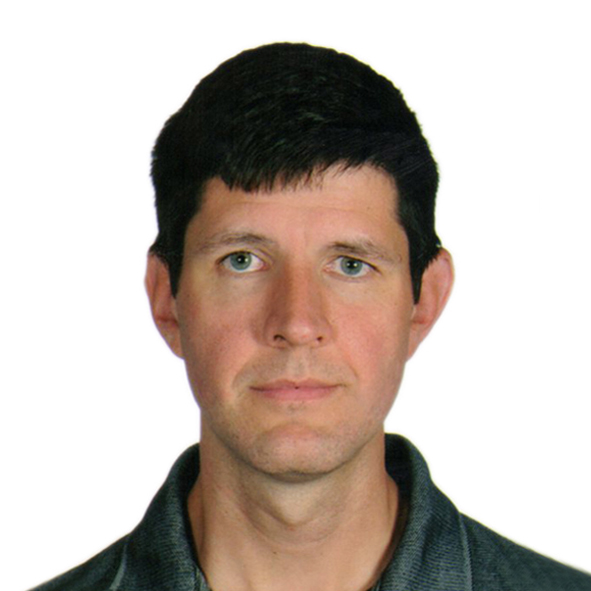
\includegraphics[width=1in,height=1.25in,clip,keepaspectratio]{Photo_Paul}}]{Paul Brown}
	(S’03–M’06)
	received the B.S. in Electrical Engineering from Iowa State University, Ames, in 2004
	and the M.S. in Electrical Engineering from the Faculty of Engineering, University of Porto, Porto, Portugal, in 2006.
	He is currently working toward a Ph.D. in Electrical and Electronics Engineering at Middle East Technical University in Ankara, Turkey, under the supervision of Murat Göl.
	He worked as a consulting electrical engineer for Peak Power Engineering in Golden, Colorado, from 2006-2013.
	He worked as a transmission system protection engineer for Nebraska Public Power District in Columbus, Nebraska, from 2013-2017.
\end{IEEEbiography}

\end{document}
